\documentclass[a4paper,14pt]{extarticle}                     % тип документа с размером шрифта 14pt

%---------------------------------------------------------------------------------------------------

%\usepackage{times}                                          % использование Times New Roman
                                                             %     (почему-то сносит все форматирование)
\usepackage[top=2cm,left=3cm,right=1cm,bottom=2cm]{geometry} % размеры полей
\usepackage[]{inputenc}                                      % эта строка нужна, чтобы документ открывался в редакторе MikTex
\usepackage[T2A]{fontenc}                                    % для поддержки русского языка
\usepackage[russian]{babel}                                  % включение русского языка
\usepackage{amsmath,amsthm,amscd,amsfonts,amssymb}           % специальные символы и т.п.
\usepackage{mathrsfs}                                        % специальные символы
\usepackage{indentfirst}                                     % отступ для начала абзаца
\usepackage{textcomp}                                        % текст в формулах
\usepackage{graphicx}                                        % подключение графики
\usepackage{listings}                                        % печать листингов
\usepackage{xcolor}                                          % использование цветов
\usepackage{caption2}                                        % для изменения стиля подписи рисунков
                                                             %     (приводит к warning-у, так что использовать только по необходимости)
\usepackage{verbatim}                                        % использование дополнительных возможностей verbatim           
\usepackage{fancybox}                                        % использование расширенного Verbatim
\usepackage[linesnumbered,boxed]{algorithm2e}                % оформление алгоритмов
\usepackage{booktabs}                                        % поддержка таблиц
\usepackage{makecell}                                        % для перевода строки внутри ячейки таблицы
\usepackage{ulem}                                            % волнистая черта снизу
\usepackage{textcomp}                                        % для коррекции положения тильды
\usepackage{longtable}                                       % многострочные таблицы
\usepackage{morefloats}                                      % подключить большее количество формул
\usepackage[section]{placeins}                               % сброс обработки флотов в конце страницы
\usepackage{float}                                           % расположение флотов прямо тут
\usepackage{setspace}                                        % чтобы менять междустрочный интервал с подписях

%---------------------------------------------------------------------------------------------------

\lstset{
aboveskip=15pt,
belowskip=15pt,
belowcaptionskip=10pt,
language={[ANSI]C++},
basewidth=0.5em,
xleftmargin=20pt,
xrightmargin=20pt,
basicstyle=\linespread{0.8}\small\ttfamily,           % 0.8 - уменьшение расстояния между строк
                                                             % linespread должен идти первым 
keywordstyle=\color[rgb]{0,0,1},
numbers=left,
numberstyle=\tiny,
stepnumber=1,
numbersep=10pt,
showspaces=false,
showstringspaces=false,
showtabs=false,
frame=trBL,
tabsize=2,
captionpos=t,
breaklines=false,
breakatwhitespace=false,
escapeinside={\%*}{*)}
}

%---------------------------------------------------------------------------------------------------

%\renewcommand{\GenericWarning}[2]{\GenericError{#1}{#2}{}{This warning has been turned into a fatal error.}} % Предупреждения -> ошибки.
\newcommand{\textapprox}{\raisebox{0.5ex}{\texttildelow}}    % положение тильды
\renewcommand{\baselinestretch}{1.5}                         % полуторный отступ между строк
\renewcommand{\captionlabeldelim}{.}                         % разделитель между номером рисунка и названием
\numberwithin{equation}{section}                             % нумерация формул по секциям
\numberwithin{figure}{section}                               % нумерация картинок по секциям
\numberwithin{table}{section}                                % нумерация таблиц по секциям
\theoremstyle{plain}                                         % стиль теорем
\newtheorem{theorem}{Теорема}[section]                       % теорема
\newtheorem{lemma}{Лемма}[section]                           % лемма
\newtheorem{definition}{Определение}[section]                % определение
\numberwithin{theorem}{section}                              % нумерация теорем по секциям
\numberwithin{lemma}{section}                                % нумерация лемм по секциям
\numberwithin{definition}{section}                           % нумерация определений по секциям

%---------------------------------------------------------------------------------------------------

\captionstyle{center}
\setlength{\abovecaptionskip}{0pt}
\setlength{\belowcaptionskip}{0pt}

%---------------------------------------------------------------------------------------------------

\begin{document}

\numberwithin{lstlisting}{section}                           % нумерация листингов по секциям
                                                             % определяем тут, так как счетчик листинга до begin{document}
                                                             % еще не существует
                                                             % https://tex.stackexchange.com/questions/441618/how-to-number-the-listings-within-sections

\title{Организация и оптимизация суперкомпьютерных вычислений в задаче моделирования обледенения поверхности}
\author{}
\date{}
\maketitle
\thispagestyle{empty}                                        % не нумеруем первую страницу

\newpage
\renewcommand{\contentsname}{Оглавление}                     % переопределяем команду перед генерацией оглавления
\tableofcontents

%---------------------------------------------------------------------------------------------------

\newpage
\section*{Введение}                      % выключить номер введения
\addcontentsline{toc}{section}{Введение} % но добавить его в оглавление

В настоящее время высокопроизводительные вычисления являются неотъемлемой составляющей научных исследований, промышленных разработок и бизнеса.
Использование высокопроизводительных вычислительных систем \cite{GOST57700HPC} находит широкое применение во всех сферах деятельности человека.

% а) переход к передовым технологиям проектирования и создания высокотехнологичной продукции
Суперкомпьютерные вычисления являются основой для развития передовых технологий проектирования и создания высокотехнологичной продукции.
В частности суперкомпьютерные вычисления применяются в авиационной и космической промышленности \cite{Kornev2021SuperAvio}, автомобилестроении \cite{Wang2020SuperAuto}, проектировании морского и железнодорожного транспорта \cite{Nikitin2018SuperShip,Solovyev2013SuperTrains}, турбин \cite{Duben2022SuperTurbine} и других высокотехнологичных изделий.
Важную роль суперкомпьютеры играют при проектировании образцов вооружения, в частности военной техники и боеприпасов \cite{Ageeva2023SuperMilitary}.
Также суперкомпьютерные вычисления незаменимы при разработке новых материалов, для изучения свойств которых требуется проводить точное атомистическое моделивование структур, состоящих из миллиардов отдельных атомов \cite{Wang2025SuperMolDyn}

% б) переход к экологически чистой и ресурсосберегающей энергетике, повышение эффективности добычи и глубокой переработки углеводородного сырья, формирование новых источников энергии, способов ее передачи и хранения
В энергетической сфере высокопроизводительные вычисления применяются для моделирования объектов генерации электроэнергии, включая атомные станции \cite{Cancemi2025SuperNuc} (в совокупности с процессами внутри ядерных реакторов \cite{Zhang2025SuperNuclear}), ветряные и приливные генераторы \cite{Quint2025SuperWind,Parrado2024SuperTidal}.
Детальное моделирование месторождений углеводородного сырья позволяет повысить эффективность добычи \cite{Usmanov2024SuperPlast}, а создание цифровых моделей месторождений и систем транспортировки \cite{Didenko2023SuperOil} приводит к снижению потерь и обеспечивает прозрачность полного жизненного цикла, начиная с добычи сырья и заканчивая реализацией конечного топлива потребителю.

% в) переход к персонализированной, предиктивной и профилактической медицине, высокотехнологичному здравоохранению и технологиям здоровьесбережения, в том числе за счет рационального применения лекарственных препаратов
Использование больших вычислительных систем позволило извлекать качественно новые данные из точного моделирования крупных органических молекул и их ансамблей \cite{Teplukhin2009SuperBigMolec}.
Во время борьбы с пандемией COVID-19 суперкомпьютерные вычисления играли передовую роль в изучении вируса и разработке вакцины \cite{Colonnelli2021SuperCovid}.
Обработка с помощью искусственного интеллекта больших массивов медицинских данных, включая истории болезней, медицинские анализы и снимки \cite{Ri2024SuperXRay}, в совокупности с геномными исследованиями в настоящее время знаменует переход к персонализированной медицине \cite{Kishore2024SuperPrecMed}.

% г) переход к высокопродуктивному и экологически чистому агро- и аквахозяйству, разработку и внедрение систем рационального применения средств химической и биологической защиты сельскохозяйственных растений и животных, хранение и эффективную переработку сельскохозяйственной продукции
Компьютерное моделирование активно используется в растениеводстве и животноводстве для повышения эффективности выработки продовольствия.
Сюда входит целый спектр применений, начиная от селекции растений и животных \cite{Ahmetshina2020SuperSelection}, мониторинга их здоровья \cite{Mourant2018SuperEpi}, разработки удобрений и кормов \cite{Irfan2016SuperFert} и заканчивая планированием графиков разведения животных и выращивания сельскохозяйственных культур \cite{Zhang2021SuperFertPlan}.

% д) противодействие техногенным, биогенным, социокультурным угрозам, терроризму и экстремистской идеологии, деструктивному иностранному информационно-психологическому воздействию, а также киберугрозам и иным источникам опасности для общества, экономики и государства, укрепление обороноспособности и национальной безопасности страны в условиях роста гибридных угроз
В связи со стремительным распространением цифровизации во всех областях современной жизни и ростом объема цифровых данных особую важность обретает задача обеспечения кибербеопасности и сохранности данных.
Злонамеренные действия в киберсреде потенциально могут привести к серьезным последствиям, включая финансовые потери, техногенные и экологические катастрофы.
Высокопроизводительные вычисления используются для исследования и созданиия новых инструментов информационной безопасности, в том числе с помощью технологий искусственного интеллекта и систем распределенного реестра \cite{Terziyska2024SuperCyber}.

% е) повышение уровня связанности территории Российской Федерации путем создания интеллектуальных транспортных, энергетических и телекоммуникационных систем, а также занятия и удержания лидерских позиций в создании международных транспортно-логистических систем, освоении и использовании космического и воздушного пространства, Мирового океана, Арктики и Антарктики
Ввиду обширности территории России и неравномерности ее заселения и инфраструктурного обеспечения, необходимо создание интеллектуальных транспортных и телекоммуникационых систем для повышения уровня связности территории.
Суперкомпьютерные вычисления применяются для проектирования и развития систем железнодорожного и авиасообщения \cite{Juntana2022SuperFlight}, обеспечения логистики морских перевозок \cite{Yan2024SuperSea}, а также для создания глобальных компьютерных сетей \cite{Abramov2025SuperNets}.

% ж) возможность эффективного ответа российского общества на большие вызовы с учетом возрастающей актуальности синтетических научных дисциплин, созданных на стыке психологии, социологии, политологии, истории и научных исследований, связанных с этическими аспектами научно-технологического развития, изменениями социальных, политических и экономических отношений
%Развитие цифровизации во всех мире затрагивает не только технические стороны жизни человека, но и социально-психологические аспекты.
%В настоящее время можно констатировать, что социально-психологический профиль человека практически полностью определяется по его цифровому следу.
%Это с одной стороны открывает возможности по моделированию социальных и политических процессов \cite{} на основе цифровых данных.
%С другой стороны, доступность цифровых данных создает уязвимости как отдельного человека, так и целых групп населения, поэтому такие угрозы также нужно %анализировать и парировать \cite{}.

% з) объективную оценку выбросов и поглощения климатически активных веществ, снижение их негативного воздействия на окружающую среду и климат, повышение возможности качественной адаптации экосистем, населения и отраслей экономики к климатическим изменениям
Так как техногенное влияние человека на окружающую среду постоянно возрастает, то в настоящее время высокопроизводительные вычисления применяются для решения задач экологии.
В частности с помощью суперкомпьютерного моделирования и глобальных моделей проводятся климатические исследования \cite{Kulkarni2024SuperClimate}, исследования мирового океана \cite{Wei2024SuperOcean}, экосистем \cite{Rahman2024SuperSpecies} и оцениваются выбросы в окружающую среду и их последствия \cite{Ostromsky2024SuperAir}.

% и) переход к развитию природоподобных технологий, воспроизводящих системы и процессы живой природы в виде технических систем и технологических процессов, интегрированных в природную среду и естественный природный ресурсооборот
В последнее время особый акцент в технологическом развитии делается на природоподобные технологии, основанные на воспроизведении систем и процессов живой природы.
Как правило, эти системы и процессы состоят из большого количества взаимодействующих элементов, которые требуют точного моделирования, что возможно только с использованием суперкомпьютеров.
К природоподобным направлениям, связанным с высокопроизводительными вычислениями, можно отнести разработку нейроморфных процессоров~\cite{Rhodes2019SuperNuero}, технологии синтеза и воспроизведения тканей и органов человека \cite{Wang2012SuperTissues}, топологическую оптимизацию в проектировании изделий и строительстве \cite{Fedchikov2024SuperBim} и другие направления.

% Суррогатные вычисления.
Широкое применение суперкомпьютерного моделирования в проектировании сложных технических систем связано с задачей выбора оптимальной конфигурации при большом количестве входных параметров.
По мере усложнения проектируемых систем и роста количества параметров возникла проблема дефицита вычислительных ресурсов, что привело к появлению концепции суррогатного моделирования\label{term:surrogate_modeling} \cite{Jiang2020Surrogate,Barcenas2023Surrogate,Catalani2024Surrogate}, то есть использования упрощенных суррогатных моделей, обученных на результатах суперкомпьютерного моделирования на ограниченных наборах данных.
Но даже использование суррогатного моделирования может лишь частично снизить потребность в вычислительных ресурсах и не умаляет актуальность проблемы эффективного их использования.

Приведенный выше, но далеко не полный перечень сфер применения высокопроизводительных вычислений отражает основные приоритеты научно-технологического развития Российской Федерации.
Развитие суперкомпьютерных технологий необходимо для обеспечения места России среди мировых технологических лидеров, поэтому вопросы создания и эффективного использования высокопроизводительных вычислительных систем являются крайне актуальными, особенно в условиях настоящего дефицита высокопроизводительных ресурсов в Российской Федерации \cite{Voevodin2021SuperRussia}.

% Расчеты в пространстве и на поверхности.
Наиболее ресурсоемкие научно-технические задачи, связанные с суперкомпьютерными расчетами, представляют собой моделирование различных физических процессов в трехмерном пространстве.
К таким задачам относятся моделирование процессов газовой динамики \cite{Lobanova2023GeneralGas}, электромагнетизма \cite{Taboada2013GeneralElectro}, термодинамики \cite{Liu2020GeneralThermo} и многих других.
При этом вычисления проводятся, как правило, с использованием расчетных сеток, которые могут описывать, как область трехмерного пространства (объемные расчетные сетки \cite{Kudryavzeva2014GeneralVolumeMesh}), так и некоторую расположенную в трехмерном пространстве поверхность (поверхностные расчетные сетки \cite{Zheleznyakova2016GeneralSurfMesh}).

Настоящая работа посвящена организации и оптимизации суперкомпьютерных вычислений, проводимых на поверхностных неструктурированных расчетных сетках\label{term:unstruct_surf_calc_mesh8}, описывающих поверхность в трехмерном пространстве, а также на объемных блочно-структурированных расчетных сетках\label{term:mesh_block_struct7}, описывающих область пространства вокруг этой поверхности.

% Задачи на поверхностях.
К числу задач суперкомпьютерного моделирования на поверхностных расчетных сетках относятся задачи внешнего обтекания \cite{Mitin2020Flow}, течения пленки жидкости по поверхности \cite{Li2014Film}, обледенения поверхности \cite{Koshelev2020Ice,Sorokin2020Ice}.
При этом задача обледенения поверхности является комплексной, так как для получения адекватной картины ледообразования необходимо учитывать множество сопряженных процессов, включая обтекание тела, выпадение на поверхность влаги и ледяных кристаллов из окружающего потока \cite{Cui2023Impingement}, взаимодействие выпадающего вещества с поверхностью \cite{Cui2021Impingement}, течение жидкости по поверхности в виде тонкой пленки или отдельных нитей \cite{Alexeenko2013Ice}, теплопроводность на поверхности \cite{Domingos2015IceHeat}, а также через слой жидкости и льда \cite{Xin2013Ice} и многие другие процессы.
Также в процессе образования слоя льда меняется сама геометрия рассматриваемой поверхности, так как форма образовавшихся ледяных наростов существенным образом влияет на все связанные процессы, что приводит к необходимости перестроения расчетных сеток.

Изучение процессов формирования ледяных наростов имеет большую практическую значимость, так как характер и размер ледяных наростов существенно влияют на летные характеристики летательного аппарата, что напрямую связано с безопасностью полетов \cite{Raj2020IntroIce}.

Настоящая работа ориентирована на проблемы суперкомпьютерного моделирования процесса обледенения поверхности, хотя результаты работы в плане организации и оптимизации вычислений примеными к другим предметным областям.

Сегодня среди зарубежного программного обеспечения для моделирования процесса ледообразования лидером является пакет инженерного проектирования ANSYS (включающий в себя модули FENSAP-ICE, DROP3D, ICE3D) \cite{Martini2022IntroIce}.
Кроме него можно назвать и другие расчетные коды, например, LEWICE \cite{Shannon2019IntroIce}, AIPAC\label{abbr:aipac} \cite{Domingos2015IceHeat}, ONERA\label{abbr:onera} \cite{Villedieu2014IntroIce}, TRAJICE \cite{Son2010IntroIce} и другие.
В России в настоящее время также разрабатывается набор алгоритмов и программного обеспечения для моделирования процесса ледообразования.
В их числе можно назвать разработку модуля iceFoam как части открытого программного обеспечения OpenFOAM\label{abbr:foam} \cite{Koshelev2020Ice}.
Среди коммерческих программных продуктов выделяется модуль IceVision в составе пакета FlowVision \cite{Sorokin2020Ice}, а также решение для моделирования ледяного покрова в составе пакета инженерного анализа ЛОГОС \cite{Galanov2021IntroIce}.

Моделирование процесса ледообразования выполняется, как правило, на поверхностных расчетных сетках и состоит из отдельных макроитераций, каждая из которых проходит в два этапа.
На первом этапе итерационно выполняется расчет интенсивности нарастания льда в рамках отдельных ячеек расчетной сетки (интенсивность ледообразования может выражаться в массе накопленного льда в ячейке за временя макроитерации, в скорости нарастания высоты ледяного покрова в узле сетки и в других характеристиках).
Для вычисления интенсивности ледообразования в элементах расчетной сетки существует множество моделей ледообразования \cite{Bartkus2018IntroIce,Zhang2017IntroIce,Pena2016IntroIce}, в которых учитываются различные состояния льда, течение жидкой пленки по поверхности, тепловые потоки, выпадение на поверхность влаги, ледяных кристаллов и переохлажденных капель \cite{Wang2023IntroIce,Liu2022IntroIce}, различные механики плавления и срыва ледяных наростов \cite{Ruan2023IntroIce} и многие другие факторы. 

\begin{figure}[ht]
\centering
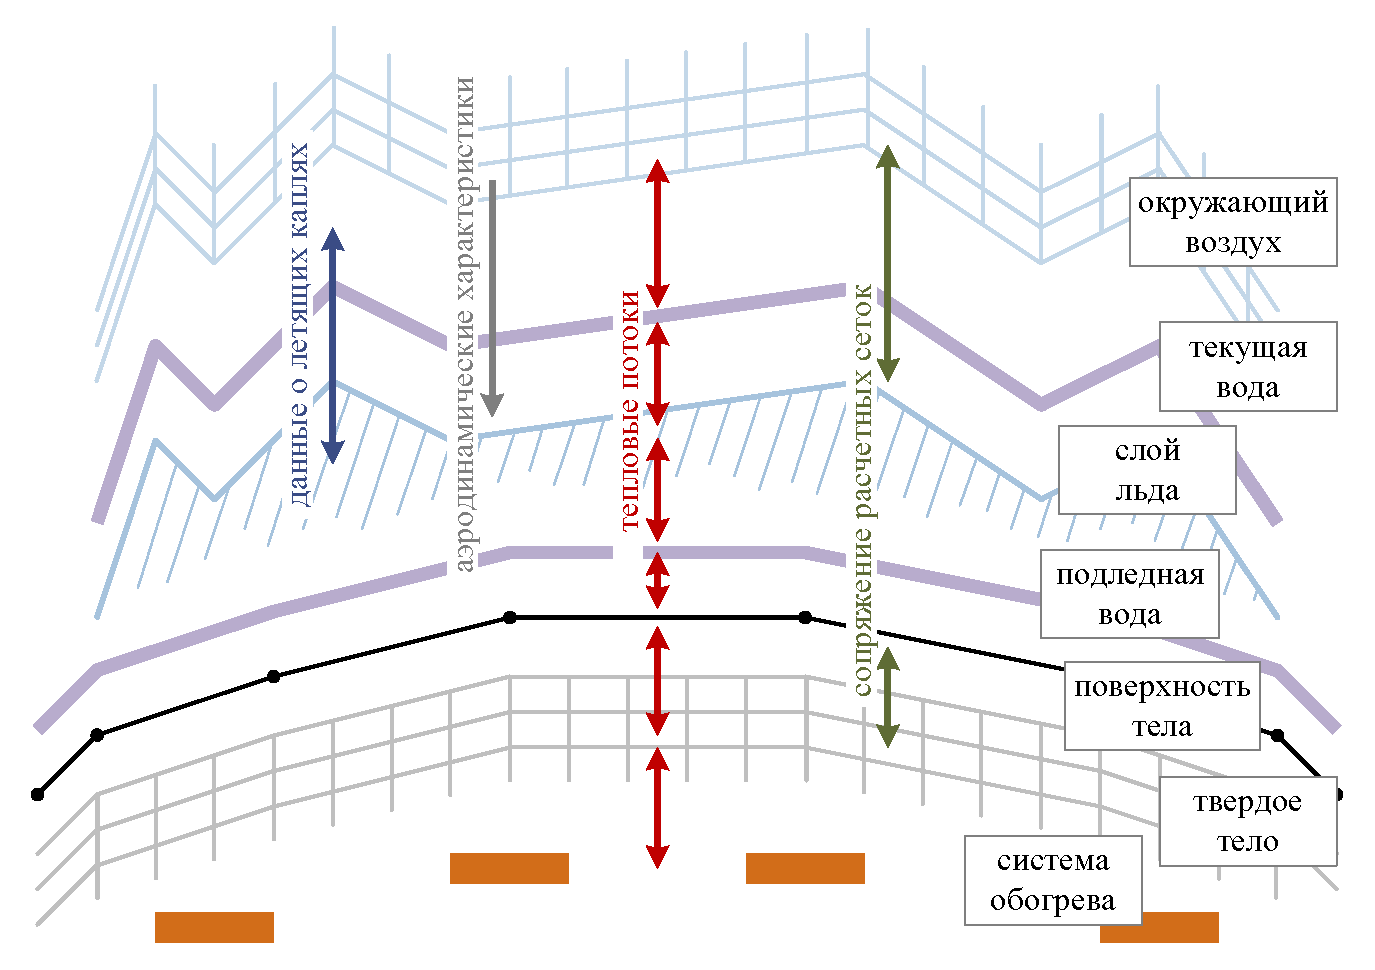
\includegraphics[width=1.0\textwidth]{pics/text_0/multi-scheme.pdf}
\singlespacing
\captionstyle{center}\caption{Многослойная модель ледообразования.}
\label{fig:text_0_multi_scheme}
\end{figure}

Во время расчета первого этапа каждая ячейка поверхностной расчетной сетки представлена в виде сложной структуры, состоящей из следующих слоев, перечисленных снизу вверх: элементы системы обогрева внутри тела -- твердое тело -- слой находящейся подо льдом жидкости -- слой льда -- текущая по поверхности льда жидкость -- окружающее воздушное пространство (см. рис.~\ref{fig:text_0_multi_scheme}).
В зависимости от используемой модели можно выделять и другие слои.
Во время выполнения расчетов осуществляется обмен потоками вещества и тепла между отдельными слоями, а также между соседними ячейками.

На втором этапе моделирования ледяных наростов выполняется перестроение поверхности обледеневающего тела.
При этом перестроение должно выполняться таким образом, чтобы изменение объема рассматриваемого тела соответствовало вычисленному объему накопленного за время макроитерации льда на первом этапе.
После перестроения поверхностной расчетной сетки необходимо произвести пересчет поля скоростей вокруг нее, так как изменение геометрии поверхности существенным образом влияет на картину обтекания.
После пересчета поля скоростей моделирование процесса обледенения может быть продолжено.

Моделирование процесса ледообразования является крайне ресурсоемким процессом, включающем в себя не только выполнение вычислений на поверхностной расчетной сетке, но и постоянный пересчет поля скоростей в окружающем пространстве.
Для выполнения моделирования образования ледяных наростов на значимом промежутке времени требуется использование существенных суперкомпьютерных ресурсов и применение методов для эффективной организации и оптимизации вычислений на всех уровнях распараллеливания: в модели с передачей сообщений, на общей памяти и на уровне отдельных инструкций.

\paragraph{Актуальность темы.} \

Дефицит суперкомпьютерных ресурсов, расширение сфер применения высокопроизводительных вычислений и усложнение моделей компьютерного моделирования отражает актуальность исследований, направленных на повышение эффективности использования суперкомпьютерных ресурсов.

Исследование процесса обледеления имеет важное научно-практическое значение для проектирования летательных аппаратов и обеспечения безопасности полетов, что говорит о необходимости разработки методов и средств для моделирования процесса обледенения.

Таким образом, организация и оптимизации суперкомпьютерных вычислений в применении к задаче моделирования обледенения поверхности, проводимых на поверхностных неструктурированных расчетных сетках, описывающих поверхность в трехмерном пространстве, а также на объемных блочно-структурированных расчетных сетках, описывающих область пространства вокруг этой поверхности, обладает актуальностью и практической значимостью.

\paragraph{Цели и задачи работы.} \

Целью работы является повышение эффективности использования суперкомпьютерных ресурсов в применении к задаче моделирования обледенения поверхности при проведении вычислений на поверхностных неструктурированных расчетных сетках, описывающих поверхность в трехмерном пространстве, а также на объемных блочно-структурированных расчетных сетках, описывающих область пространства вокруг этой поверхности.

Для достижения поставленной цели в диссертационной работе необходимо решить следующие задачи:

\begin{enumerate}
\item Разработать и реализовать архитектуру поверхностной неструктурированной расчетной сетки\label{term:unstruct_surf_calc_mesh9} с поддержкой декомпозиции для распараллеливания вычислений и перестроения для моделирования эволюции поверхности в процессе ледообразования.
\item Разработать и реализовать архитектуру объемной блочно-структуриро-ванной расчетной сетки\label{term:mesh_block_struct8} с поддержкой декомпозиции для распараллеливания вычислений.
\item Разработать и реализовать механизм сопряжения поверхностной неструктурированной расчетной сетки с объемной блочно-структурированной расчетной сеткой для расчета процесса обтекания поверхности в условиях изменения геометрии.
\item Разработать и реализовать методы декомпозиции и распределения вычислительной нагрузки для распараллеливания вычислений на поверхностной неструктурированной расчетной сетке и объемной блочно-струк-турированной расчетной сетке в модели распараллеливания с передачей сообщений.
\item Разработать и реализовать методы распараллеливания вычислений на поверхностной неструктурированной расчетной сетке и объемной блочно-структурированной расчетной сетке в модели распараллеливания на общей памяти.
\item Разработать и реализовать методы низкоуровневого распараллеливания вычислений с помощью векторизации программного кода.
\end{enumerate}

\paragraph{Методы исследования.} \

TODO

\paragraph{Научная новизна и практическая значимость.} \

TODO

Описанные в работе методы и алгоритмы апробированы на суперкомпьютерах Межведомственного суперкомпьютерного центра Российской академии наук и Национального центра <<Курчатовский институт>> и реализованы в рамках инструментов суперкомпьютерного моделирования, на которые оформлены 7 свидетельств о государственной регистрации программы для ЭВМ.
В частности, разработанные в рамках диссертации методы перестроения поверхностной неструктурированной расчетной сетки, а также методы повышения эффективности суперкомпьютерных расчетов на ней нашли свое отражение в программном модуле компьютерного моделирования процесса обледенения элементов авиационных силовых установок <<Кристалл>> \cite{CertGoryachev2023Crys,CertGoryachev2020Crys}.
Разработаны инструменты подготовки поверхностной неструктурированной расчетной сетки и объемной блочно-структурированной расчетной сетки для суперкомпьютерных вычислений \cite{CertRybakov2021PrepUnstruct,CertRybakov2020PrepStruct} и библиотека организации вычислений на поверхностной неструктурированной расчетной сетке \cite{CertRybakov2024Surf}.
Разработаны программные коды для векторизации высокопроизводительных вычислений \cite{CertRybakov2019AVX,CertRybakov2023Mon}.

\paragraph{Основные положения, выносимые на защиту.} \

\begin{enumerate}
\item Предложен метод перестроения поверхностной неструктурированной расчетной сетки с использованием окрестностей ячеек для задачи ледообразования.
\item Предложен метод устранения самопересечений поверхностной неструктурированной расчетной сетки.
\item Предложен алгоритм распределения вычислительной нагрузки при расчетах на объемной блочно-структурированной расчетной сетке с дроблением блоков.
\item Предложен алгоритм сглаживания границ доменов при декомпозиции поверхностной неструктурированной расчетной сетки.
\item Проведен анализ распараллеливания плотных вычислений на общей памяти и обоснован выбор вычислительной системы с точки зрения эффективности распараллеливания.
\item Введено понятие плоского цикла, определены основные его характеристики и обоснован подход к векторизации, основанный на создании программного кода с помощью композиции плоских циклов.
\item Предложены методы векторизации плоских циклов, на основе которых продемонстрирована эффективность векторизации на ряде научно-практических задач.
\end{enumerate}

\paragraph{Апробация работы.} \

Материалы диссертации докладывались на следующих конференциях и семинарах:

\begin{itemize}
\item V Национальный Суперкомпьютерный Форум (НСКФ-2016), Россия, Переславль-Залесский, Институт программных систем им. А.~К.~Айламазяна, 29 ноября -- 2 декабря 2016 г.
\item VII Национальный Суперкомпьютерный Форум (НСКФ-2018), Россия, Переславль-Залесский, Институт программных систем им. А.~К.~Айламазяна, 27-30 ноября 2018 г.
\item X Национальный Суперкомпьютерный Форум (НСКФ-2021), Россия, Переславль-Залесский, Институт программных систем им. А.~К.~Айламазяна, 30 ноября -- 3 декабря 2021 г.
\item I Международная научная конференция <<Конвергентные когнитивно-информационные технологии>>, Россия, Москва, Московский государственный университет им. М.~В.~Ломоносова, 25-26 ноября 2016 г.
\item III Международная научная конференция <<Конвергентные когнитивно-информационные технологии>>, Россия, Москва, Московский государственный университет им. М.~В.~Ломоносова, 22-25 ноября 2018 г.
\item XVI Международная конференция <<Супервычисления и математическое моделирование>>, Россия, Саров, Российский федеральный ядерный центр -- Всероссийский научно-исследовательский институт экспериментальной физики, 3-7 октября 2016 г.
\item VI всероссийская конференция <<Вычислительный эксперимент в аэроакустике>>, Россия, Светлогорск, организатор -- Институт прикладной математики им. М.~В.~Келдыша РАН, 19-24 сентября 2016 г.
\item Слет разработчиков отечественных CFD кодов (CFD Weekend 2023), Россия, Москва, Институт прикладной математики им. М.~В.~Келдыша, 9-10 декабря 2023 г.
\item Слет разработчиков отечественных CFD кодов (CFD Weekend 2022), Россия, Москва, Институт прикладной математики им. М.~В.~Келдыша, 3-4 декабря 2022 г.
\item The Intel Xeon Phi users group Russia annual meeting (IXPUG Russia-2017), // Joint Supercomputer Center of the Russian Academy of Sciences (JSCC RAS), Russia, Moscow, 1-2 June 2017.
\end{itemize}

\paragraph{Содержание.} \

TODO

%---------------------------------------------------------------------------------------------------

\newpage
\section*{Глава 1. Геометрические методы организации \\ работы с неструктурированной поверхностной \\ расчетной сеткой} % выключить номер первой главы
\addcontentsline{toc}{section}{Глава 1. Геометрические методы организации работы с неструктурированной поверхностной расчетной сеткой}                                                                                                           % но добавить ее в оглавление
\addtocounter{section}{1}                                                                                         % а теперь и счетчик продвинуть
\setcounter{subsection}{0}
\setcounter{figure}{0}
\setcounter{equation}{0}
\setcounter{table}{0}
\setcounter{theorem}{0}
\setcounter{lemma}{0}
\setcounter{definition}{0}

\input text_1_geo_prim.tex
\input text_1_remesh_2d.tex
\input text_1_remesh_3d.tex
\input text_1_remesh_common_envelope.tex
\input text_1_int.tex
\input text_1_gas_dyn.tex
\input text_1_immersed_boundary_method.tex

\subsection{Выводы из главы}

TODO

%---------------------------------------------------------------------------------------------------

\newpage
\section*{Глава 2. Методы распаралеливания вычислений с передачей сообщений}                      % выключить номер первой главы
\addcontentsline{toc}{section}{Глава 2. Методы распаралеливания вычислений с передачей сообщений} % но добавить ее в оглавление
\addtocounter{section}{1}                                                                                                % а теперь и счетчик продвинуть
\setcounter{subsection}{0}
\setcounter{figure}{0}
\setcounter{equation}{0}
\setcounter{table}{0}
\setcounter{theorem}{0}
\setcounter{lemma}{0}
\setcounter{definition}{0}
\setcounter{lstlisting}{0}

\input text_2_1_qual.tex
\input text_2_2_block.tex
\input text_2_3_getero.tex
\input text_2_4_withcut.tex
\input text_2_5_decompsurf.tex
\input text_2_6_smooth.tex
\input text_2_7_genetic.tex
\input text_2_8_scaling.tex

\subsection{Выводы из главы}

TODO

%---------------------------------------------------------------------------------------------------

\newpage
\section*{Глава 3. Методы распараллеливания \\ вычислений на общей памяти}                      % выключить номер первой главы
\addcontentsline{toc}{section}{Глава 3. Методы распараллеливания вычислений на общей памяти} % но добавить ее в оглавление
\addtocounter{section}{1}                                                                    % а теперь и счетчик продвинуть
\setcounter{subsection}{0}
\setcounter{figure}{0}
\setcounter{equation}{0}
\setcounter{table}{0}
\setcounter{theorem}{0}
\setcounter{lemma}{0}
\setcounter{definition}{0}
\setcounter{lstlisting}{0}

\input text_3_graph_prim.tex
\input text_3_edge_coloring.tex
\input text_3_omp1.tex
\input text_3_omp2.tex

\subsection{Выводы из главы}

TODO

%---------------------------------------------------------------------------------------------------

\newpage
\section*{Глава 4. Методы векторизации программного \\ кода для повышения его производительности}                      % выключить номер первой главы
\addcontentsline{toc}{section}{Глава 4. Методы векторизации программного кода для повышения его производительности} % но добавить ее в оглавление
\addtocounter{section}{1}                                                                                           % а теперь и счетчик продвинуть
\setcounter{subsection}{0}
\setcounter{figure}{0}
\setcounter{equation}{0}
\setcounter{table}{0}
\setcounter{theorem}{0}
\setcounter{lemma}{0}
\setcounter{definition}{0}
\setcounter{lstlisting}{0}

\input text_4_01_vec_description.tex
\input text_4_02_small_matr.tex
\input text_4_03_spec_matr.tex
\input text_4_04_flat.tex
\input text_4_05_ibm.tex
\input text_4_06_vec_loc_branch.tex
\input text_4_07_vec_mrg_under_cond.tex
\input text_4_08_vec_check_mask.tex
\input text_4_09_vec_comb_mask.tex

% Опционально можно добавить, тут страницы на 2-3.
%\input text_4_tozh.tex

\input text_4_10_mesh_intersect.tex
\input text_4_11_vec_riemann.tex
\input text_4_12_vec_irreg.tex
\input text_4_13_vec_integer.tex

\subsection{Выводы из главы}

\begin{figure}[ht]
\centering
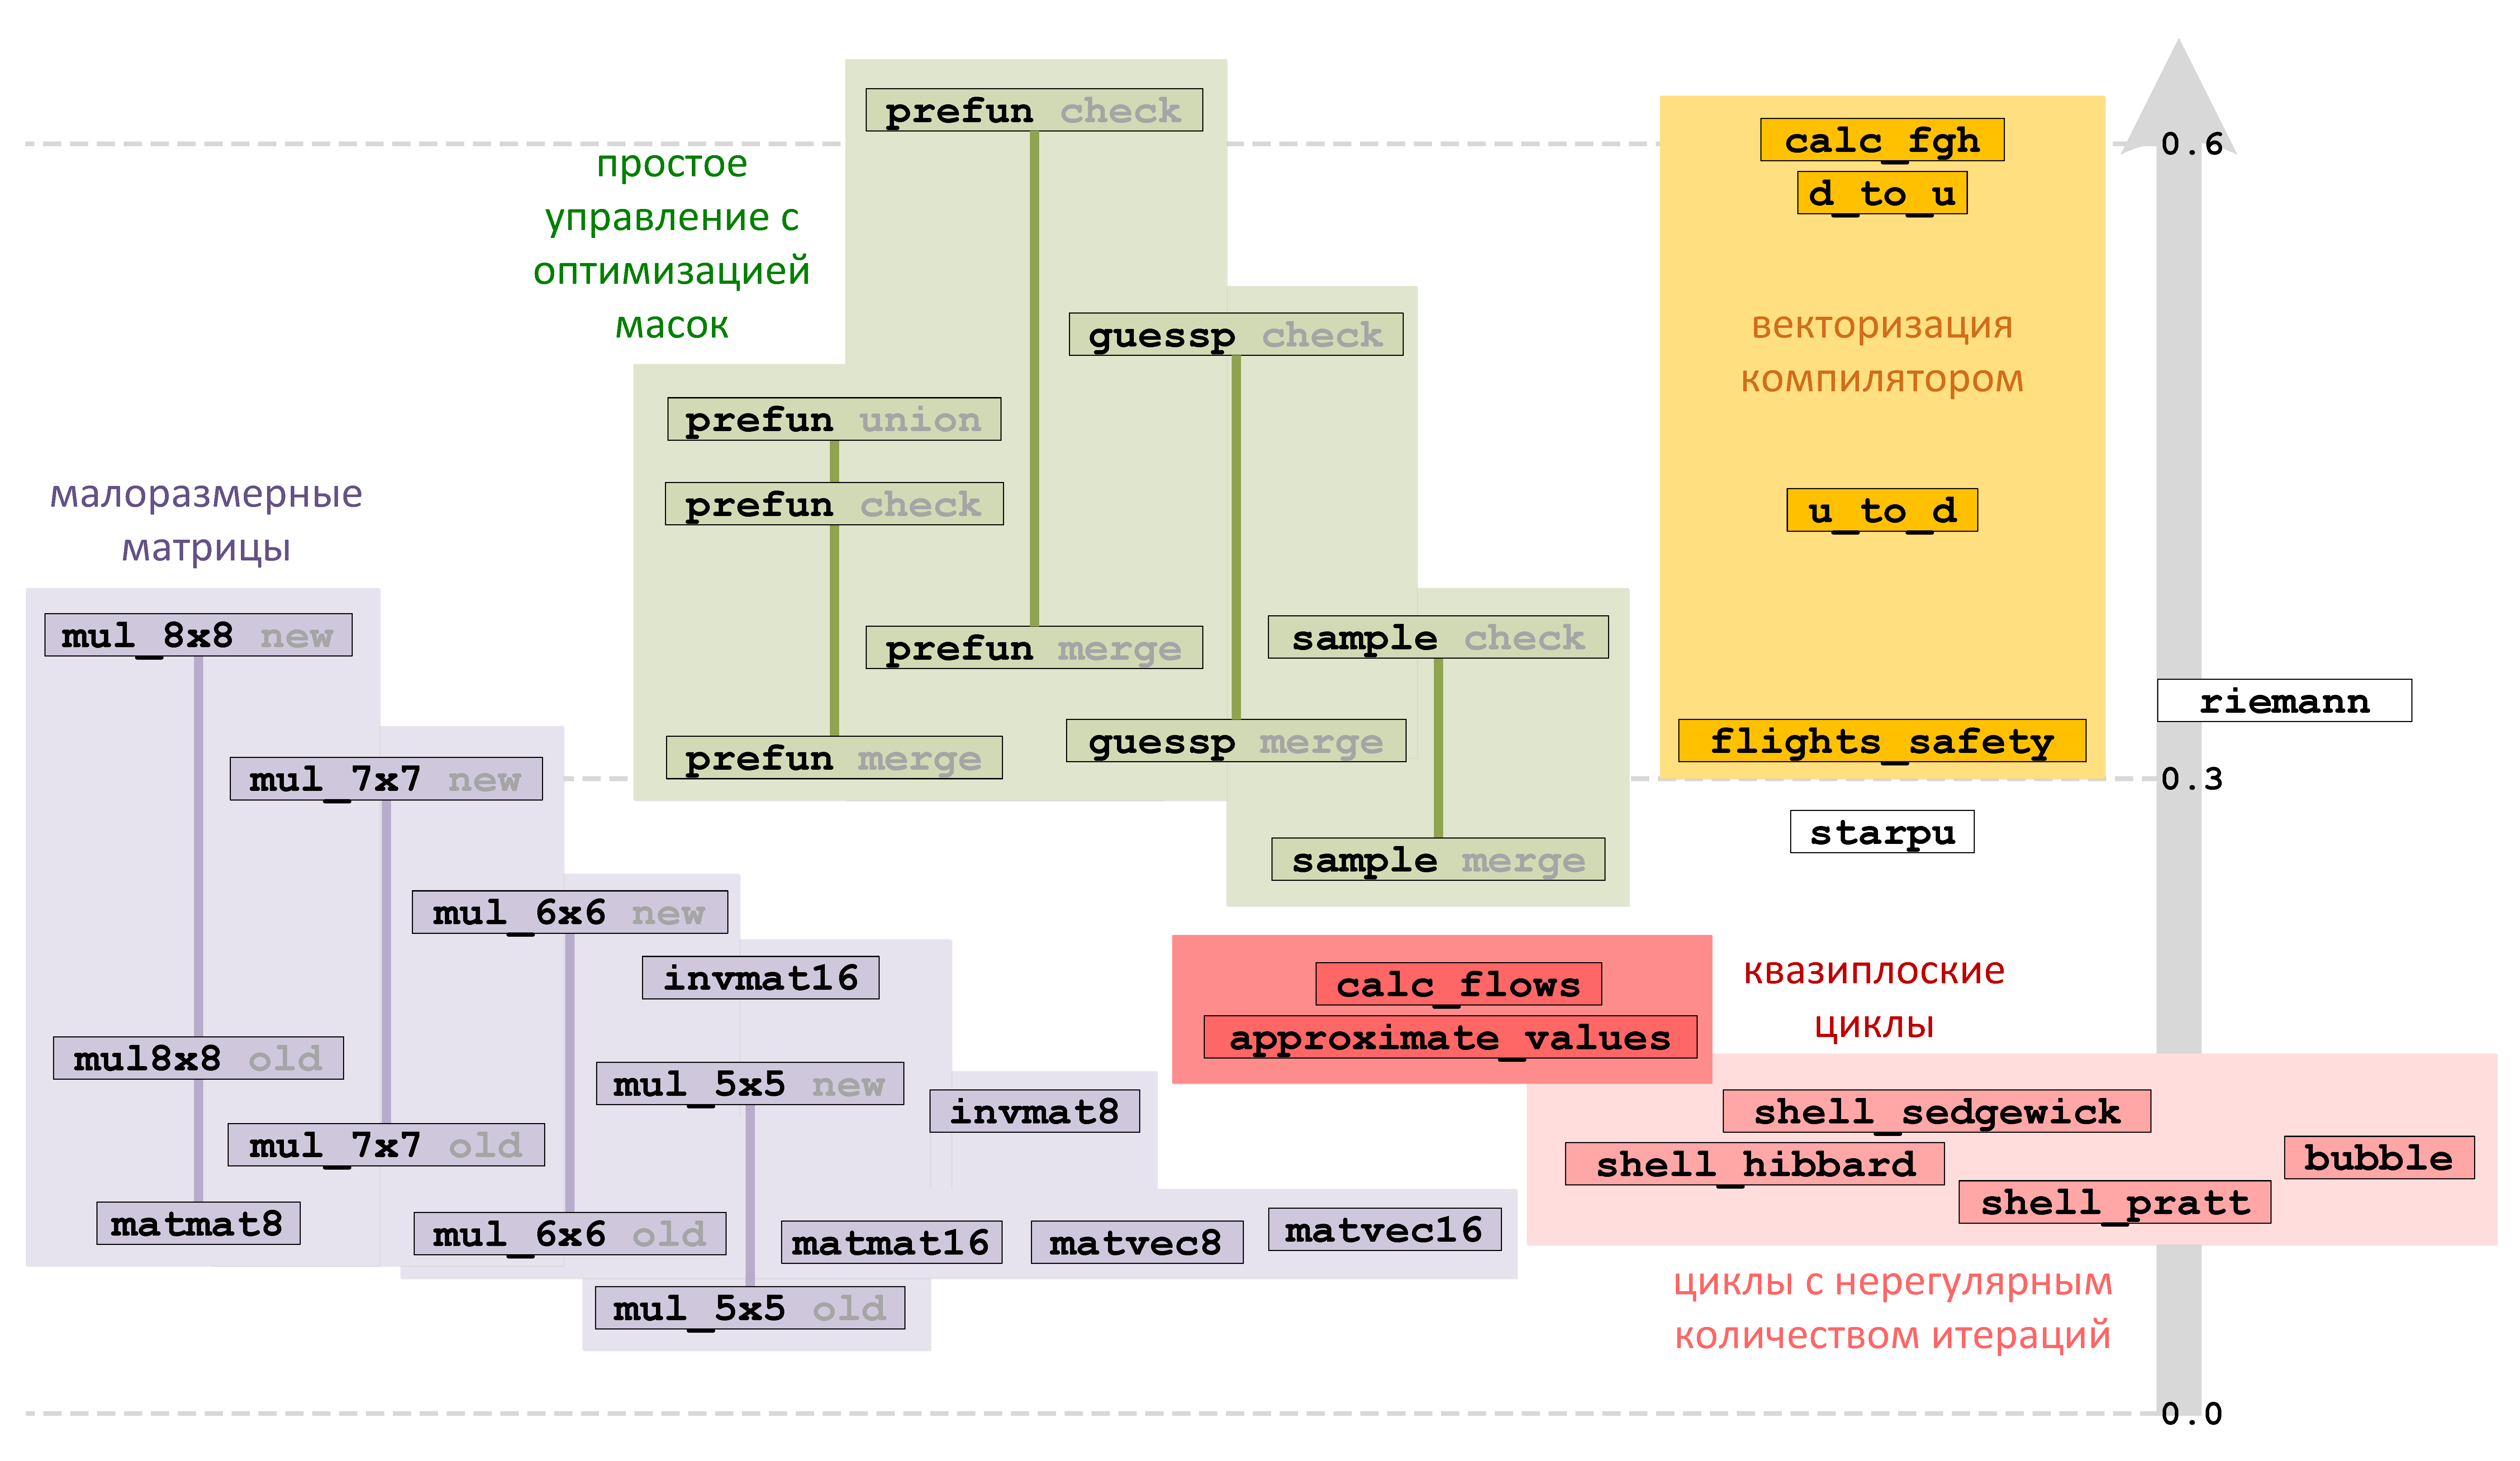
\includegraphics[width=1.0\textwidth]{./pics/text_4_fin/map_cut.pdf}
\singlespacing
\captionstyle{center}\caption{Карта эффективности векторизации.}
\label{fig:text_4_fin_map}
\end{figure}

Векторизация\label{term:vectorization7} является важной низкоуровневой оптимизацией программного кода, с помощью которой можно достичь кратного ускорения суперкомпьютерных приложений.
Все основные современные микропроцессорные архитектуры поддерживают векторные вычисления, причем наблюдается тенденция на увеличение размера вектора (на сегодняшний день максимальная длина равна 512 битам, но уже сейчас логически эта длина не ограничена, учитывая наборы векторных инструкций с переменной длиной вектора).

Сейчас наиболее перспективным набором векторных инструкций является набор AVX-512\label{abbr:avx9}, так как в нем поддержана возможность выборочной обработки элементов векторов с помощью векторных масок\label{term:vector_mask9}.
Эта уникальная возможность позволяет векторизовать сложный программный контекст, содержащий команды передачи управления, гнезда циклов и вызовы функций.

В этой главе были рассмотрены и предложены новые методы векторизации программного кода.
На рис.~\ref{fig:text_4_fin_map} приведена карта сравнения программного контекста различного вида по эффективности векторизации $e_{vec}$.
На этом рисунке схожие по свойствам тестовые примеры объединены в одной цветовой гамме.
Многие из представленных тестовых примеров векторизации программного кода были использованы при численном решении задач обледенения и газовой динамики.

В разделах \ref{sec:text_4_small_matr}, и \ref{sec:text_4_spec_matr} продемонстрированы подходы к векторизации матричных операций малой размерности.
При выполнении векторизации программного кода необходимо уметь находить наборы однотипных операций для объединения их в векторные операции над векторными наборами данных.
При этом полнота использования элементов векторных данных в вычислениях, выраженная в высокой плотности векторных масок\label{term:vector_mask_density7}, напрямую влияет на эффективность векторизации\label{term:vec_eff8} (см. риc.~\ref{fig:text_4_fin_map}, малоразмерные матрицы).

В разделе \ref{sec:text_4_flat} введено понятие плоского цикла\label{term:flat_loop6}, с помощью которого предпринимается попытка унифицировать процесс объединения однотипных операций в векторные инструкции путем записи тела плоского цикла в предикатной форме\label{term:predicate_view5} с последущей векторизацией с помощью замены скалярных операций векторными аналогами.
Можно констатировать, что плоский цикл может быть векторизован при практически произвольном виде его тела (тело может содержать сложное управления, гнезда циклов, вызовы функций).

В разделе \ref{sec:text_4_ibm} приведено описание подхода, как вычисления могут быть представлены в виде композиции плоских циклов с относительно простым телом, после чего успешно векторизованы оптимизирующим компилятором в автоматическом режиме (см. рис.~\ref{fig:text_4_fin_map}, \texttt{calc\_fgh}, \texttt{calc\_d\_to\_u}, \texttt{calc\_u\_to\_d}).
При этом рассматривается предпочтительный способ организации хранения данных в виде <<набора массивов>> и оптимизация расщепления гнезда циклов по условию\label{term:loop_split_by_cond4} для уменьшения количества операций передачи управления внутри плоского цикла.
Отмечено, что цикл, не являющийся в полной мере плоским (квазиплоский цикл)\label{term:flat_kvazy_flat2}, также может быть успешно векторизован, но с некоторой потерей производительности (см. рис.~\ref{fig:text_4_fin_map}, \texttt{calc\_flows}).

Так как основной преградой к эффективной векторизации является наличие операций передачи управления внутри тела плоского цикла (операция передачи управления не может быть векторизована), то в разделе \ref{sec:text_4_loc_branch} рассматриваются оптимизации, направленные на избавление от условий внутри цикла.
Рассматривается оптимизация выноса маловероятного региона из цикла\label{term:meth_vec_del_low_prob_regions3} и поставлен эксперимент по определению эффективности автоматической векторизации при использовании этой оптимизации (см. рис.~\ref{fig:text_4_fin_map}, \texttt{flights\_safety}).
Приведено описание оптимизации <<черная дыра>>\label{term:blackhome_optimization2} по выделению вероятного пути исполнения в теле плоского цикла.

В разделе \ref{sec:text_4_vec_mrg_under_cond} приведено описание и теоретическая оценка общего подхода к избавлению от операций передачи управления и слиянию путей исполнения\label{term:meth_vec_merge4} в теле плоского цикла с помощью векторных инструкций blend.

В разделе \ref{sec:text_4_vec_check_mask} описывается простая операция проверки векторных масок на пустоту\label{term:meth_vec_check4}, которая оказывает наибольший прирост производительности при векторизации простого программного контекста (см. рис.~\ref{fig:text_4_fin_map}, функции с пометкой \texttt{check}).

В разделе \ref{sec:text_4_comb_mask} предлагается метод объединения векторных масок\label{term:meth_vec_union3}, позволяющих одновременно исполнять блоки векторных инструкций с непересекающимися масками (см. рис.~\ref{fig:text_4_fin_map}, \texttt{prefun union}).
Также предлагается метод комбинирования векторных масок\label{term:meth_vec_comb2}, позволяющий одновременно исполнять блоки векторных инструкций с пересекающимися масками.

Остальные разделы посвещены методам векторизации гнезд циклов, в которых один из циклов является плоским.

Наиболее простым случаем является векторизаци гнезда циклов с постоянным количеством итераций, так как в этом случае условие выхода из цикла не требует векторизации.
Этот случай рассмотрен в разделе \ref{sec:text_4_vec_mesh_intersect} и продемонстрировал лучшую эффективность среди примеров векторизации гнезд циклов (см. рис~\ref{fig:text_4_fin_map}, \texttt{tri\_box\_intersect}).

В разделе \ref{sec:text_4_vec_riemann} расмсотрен пример векторизации гнезда циклов с непостоянным количеством итераций для расчетной задачи, в которой условие выхода из цикла на разных итерациях плоского цикла меняется медленно.
Векторизация такого гнезда циклов возможна с помощью векторизации условия выхода из цикла, и эффективность векторизации оказывается ниже, чем в примере с постоянным количеством итераций (см. рис.~\ref{fig:text_4_fin_map}, \texttt{starpu}).

Наиболее сложным для векторизации случаем является векторизация гнезд циклов с нерегулярным количеством итераций.
Такой программый контекст рассмотрен в разделах \ref{sec:text_4_vec_irreg} (вещественные вычисления) и \ref{sec:text_4_integer} (целочисленные вычисления).
При этом внутри итерации плоского цикла векторизуемые условия оказываются непредсказуемыми, что приводит к понижению плотности векторных масок\label{term:vector_mask_density8} в векторных инструкциях и падению производительности (см. рис.~\ref{fig:text_4_fin_map}, циклы с нерегулярным количеством итераций).
Такой программный контекст характерен для дискретных задач и он демонстрирует наиболее низкую эффективность векторизации.

%---------------------------------------------------------------------------------------------------

\newpage
\section*{Заключение}                                        % выключить номер заключения
\addcontentsline{toc}{section}{Заключение}                   % но добавить его в оглавление

%---------------------------------------------------------------------------------------------------

\input text_abbr.tex         % список сокращений
\input text_term.tex
\input text_bibliography.tex % список используемой литературы

%---------------------------------------------------------------------------------------------------

\end{document}
